\documentclass[12pt,a4paper]{article}
\usepackage[utf8]{inputenc}
\usepackage[english]{babel}
\usepackage{xstring}
\usepackage{siunitx}
\usepackage{amsmath}
\usepackage{graphicx}
\usepackage[nottoc]{tocbibind} %Adds "References" to the table of contents
\usepackage{hyperref}
\usepackage[toc]{glossaries}
\usepackage{textcomp}
\usepackage{csvsimple}
\usepackage{pgfplotstable}
\pgfplotsset{compat=1.9}% supress warning
\usepackage{longtable}
\usepackage{xcolor,colortbl}
\usepackage{listings}
\usepackage[toc,page]{appendix}
\usepackage{fancyvrb}
\usepackage{tikz}


\lstset{ %
language=C++,           % choose the language of the code
numbers=left,           % where to put the line-numbers
numberstyle=\tiny,      % the size of the fonts that are used for the line-numbers
basicstyle=\footnotesize    % the size of the fonts that are used for the line-numbers
}

\newcommand{\mc}[2]{\multicolumn{#1}{c}{#2}}
\definecolor{Gray}{gray}{0.85}
\definecolor{LightCyan}{rgb}{0.88,1,1}

\newcolumntype{A}{>{\columncolor{Gray}}c}
\newcolumntype{B}{>{\columncolor{white}}c}

% MODIFY NUMBERING OF TABLES AND PICTURES
\usepackage{chngcntr}
\counterwithin{table}{section}
\counterwithin{figure}{section}
\counterwithin{equation}{section}
\usepackage{floatrow}
\floatsetup[table]{capposition=top}

% HEADINGS AND MARGINS 
\usepackage{geometry}
 \geometry{
 a4paper,
 left=25mm,
 right=25mm,
 top=25mm,
 bottom=25mm,
 headheight=15mm,
 footskip=15mm,
 }
 

% PAGE STYLE SECTION
\usepackage{fancyhdr}
\pagestyle{fancy}
\renewcommand\sectionmark[1]{\markboth{\thesection\ #1}{}}
\fancyhf{}
\fancyhead[C]{\bfseries\leftmark}
\fancyfoot[C]{\bfseries\thepage}
\renewcommand{\headrulewidth}{0.5pt}% suppress the header rule

% INDENTATATIONS
\usepackage{indentfirst}
\setlength{\parindent}{0.75cm}

% FONT
\usepackage{times}

% UNIVERISTY LOGO TRIGGER
\usepackage{graphicx}

% TITLES OF PARTICULAR SECTIONS
\usepackage{titlesec}

\titleformat{\section}
    {\large\bfseries\itshape}
    {\thesection}
    {1em}
    {\MakeUppercase}
\titleformat{\subsection}
    {\large\bfseries\itshape}
    {\thesubsection}
    {1em}
    {}
\titleformat{\subsubsection}
    {\large\bfseries\itshape}
    {\thesubsubsection}
    {1em}
    {}
\titleformat{\paragraph}
    {\large\bfseries}
    {\theparagraph}
    {1em}
    {}
\titleformat{\subparagraph}
    {\large\bfseries}
    {\thesubparagraph}
    {1em}
    {}

\begin{document}

\begin{titlepage}
    \centering
    
\includegraphics[width=7cm]{logo.jpg} % also works with 
    \vskip1cm
    {\Large
        SILESIAN UNIVERSITY OF TECHNOLOGY\\
        FACULTY OF ELECTRICAL ENGINEERING\\
        \vskip0.5cm
        Department of Power Electronics, Electrical Drives and Robotics\\
    }
    \vskip1cm
    {\bfseries\huge
    Master's thesis\\
    }
    \vskip1cm
    {\bfseries\large
    To be determined \\
    }
    \vskip2cm
    {\large
    \begin{tabular}{p{4cm} p{10cm}}
    Student: & {\bfseries\Large Igor Aleksander JANKIEWICZ}\\
    Transcript no.: & 285947\\
        &   \\
    Type of studies: & Extramural studies (MSc programme)\\
    Field of study: & Electrical Engineering\\
    Programme: & To be determined\\
        &   \\
    Supervisor: & PhD. EEng. Andrzej Latko\\
    \end{tabular}
    }
    \vskip2.5cm
    {\large
    Gliwice 2020}
\end{titlepage}
\newpage\null\thispagestyle{empty}\newpage
\tableofcontents
\newpage\null\thispagestyle{empty}\newpage

\section{Introduction}
This Master's thesis is focused on Piezoelectic Energy Harvesting in general. Apart from the explanation of the actual energy scavenging process, it also covers a design of a proper data acquisition system used for evaluation and development of piezoelectric-based generators.
\par

\subsection{Motivation}
Nowadays, electrical energy itself is taken for granted by most of the people. It may be a result of the fact that most of household appliances and daily use items require that energy to operate. Moreover, almost any of our tasks requite a proper illumination, Internet access or simply the outlet to liven any tool we might need at the moment. To conclude, it is almost impossible to imagine our life without an access to the power gird.
\par
On the other hand, it is important to keep in mind that most of electricity we utilize comes from non-renewable fuels such as coal, liquid gas or crude oil. At some point, humankind is to face a problem of insufficient deposits of these materials, therefore it tremendously important to look for alternatives. Of course, people have already taken advantage of water, wind or solar radiation, what is proven by the existence of many green power plants around the world. Unfortunately, one of the major problems faced by all of there plans is the intermittent access to the energy source. Moreover, there are many places that does not allow to use any of these well explored solutions, forcing engineers to look for new ones. This could be a reason why vibrational energy is getting more awareness over last years.
\par

Energy harvesting from vibration gives many new possibilities, especially in IoT (Internet of Things) applications, as well as in industrial environment. The second application seems particularly tempting, as in many industrial applications, there is a lot of vibration involved, what gives a wide scope for custom sensor development. Piezoelectric harvesters are relatively compact, therefore it is possible to install them in inaccessible places. Moreover, they are robust, providing that a proper enclosure is used for mechanical protection.
\par

All of mentioned factors gained author's interest, and in the event prompted to work on this subject within the confines of this thesis.
\par

\subsection{Objective of a Master's thesis}
The main goal stated by the author is to examine a potential of vibration-based energy scavenging. In order to do so, number of different aspects need a thorough investigation. Undeniably, much of the focus would be put on the energy harvester itself. Nevertheless, a proper measurement and data acquisition system is also an important aspect throughout the entire work, since it will allow confirm or deny thesis statements posed during the research. In addition, the design process of the mentioned device would allow a more in-depth analysis of the piezoelectric generator itself, since the understanding of its operation is the only way to come up with a suitable measurement system.
\par
Returning to the piezoelectric generator, the first thing to look at is the theory behind the piezoelectric effect. Then, there would be a description of the piezoelectric cantilever  and its properties. Subsequently, the complete mechanical and electrical model would be studied.
\par

Once the required theory is introduced, it is possible to focus exactly on the topic.

\section{What is Energy Harvesting?}
Energy Harvesting is a process of using ambient energy by converting it into a usable form, i.e. electricity or heat. It is important to point out that energy harvesting has been around for quite a long time, since solar panels, wind turbines and water turbines are in constant use for a few decades, providing people with environmentally clean energy \cite{EnHv1}.
\vskip 5mm
There are some important issues related to any energy source that could be potentially used for harvesting. First of all, it is crucial to evaluate intensity and availability of that source. Subsequently, one should find out a cost-effectiveness of the solution as well as the influence of the harvesting process on the primary energy source \cite{EnHv1}.\par
\vskip 5mm
Vibration-based Energy Harvesting incorporates a number of different fields of study, i.e. material science, mechanics or electrical engineering, just to name a few. Last sentence implies that the analysis of a piezoelectric generator itself is not a straightforward process. The electromechanical response of this device relies thoroughly on the source of ambient energy \cite{EnHv2}.\par

\begin{figure}[h!]
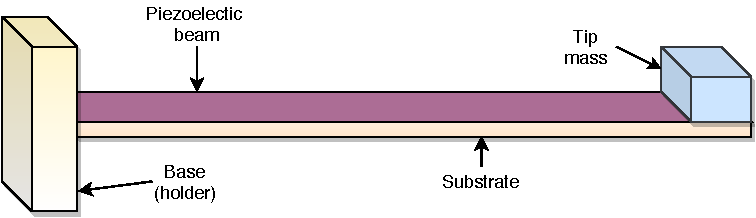
\includegraphics[scale=1]{beam1.pdf}
\end{figure}

\begin{table}[ht]
\small
\begin{center} 
\begin{tabular}{|c|c|c|c|l|}
\hline 
\textbf{Type} & \textbf{Conditions} & \textbf{Power Density} & \textbf{Area or Volume} & \textbf{Energy/Day} \\ 
\hline 
\hline
Vibration & $1m/s^2$ & $100\mu W/cm^3$ & $1cm^2$ & $8.64J$ (continuous vibration) \\ 
\hline 
Solar & Outdoors & $7500\mu W/cm^2$ & $1cm^2$ & $324J$ (sunny half a day) \\ 
\hline 
Solar & Indoors & $100\mu W/cm^2$ & $1cm^2$ & $4.32J$ (sunny half a day) \\ 
\hline 
Thermal & $\Delta T = 5 ^{\circ} C$ & $60\mu W/cm^2$ & $1cm^2$ & $2.59J$ (heat available for half a day) \\ 
\hline 
\end{tabular} 
\end{center}
\caption{Common data for some of Energy Harvesting Sources \cite{EnHv1}}
\label{tab:typdat}
\end{table}

\section{Measurement setup design}

A proper measurement process is a crucial part of this project. Having said that, a custom data acquisition board is to be designed.
\par

First of all, it is vital to highlight most important features required to achieve desired performance. There are four major aspects that have to be taken into account, namely, the ADC resolution as well as the input voltage range, the bandwidth and high input impedance of the analog front-end. Apart from that, one should take care of easy interfacing to personal computer, thus compact size and USB interface would be considered as huge assets.
\par
The previous paragraph introduced briefly main functionalities of the target device. It is quite easy to notice that there would be a lot of trade-offs to consider through the design process. Compact size and the complex analog circuitry usually do not mix, especially when planning to get a device of USB mass storage size. These facts are forcing the designer to look for a microcontroller that provides decent ADCs, also in terms of the sampling rate. Since the project is dealing with piezoelectric generators, there is always a risk of relatively high voltages at the input terminals, especially when harvesters are not connected to any load. To face this problem, the data acquisition board would be equipped with two different means of protection. The first one takes care of the input stage of the device. The second one is a classic galvanic isolation between the microcontroller (as well as the analog front end) and the personal computer. This way, there is no risk of damaging host devices utilizing the data acquisition system. The summary of the above-mentioned description is presented in the Figure~\ref{fig:meas_overview}.\par

\begin{figure}[h!]
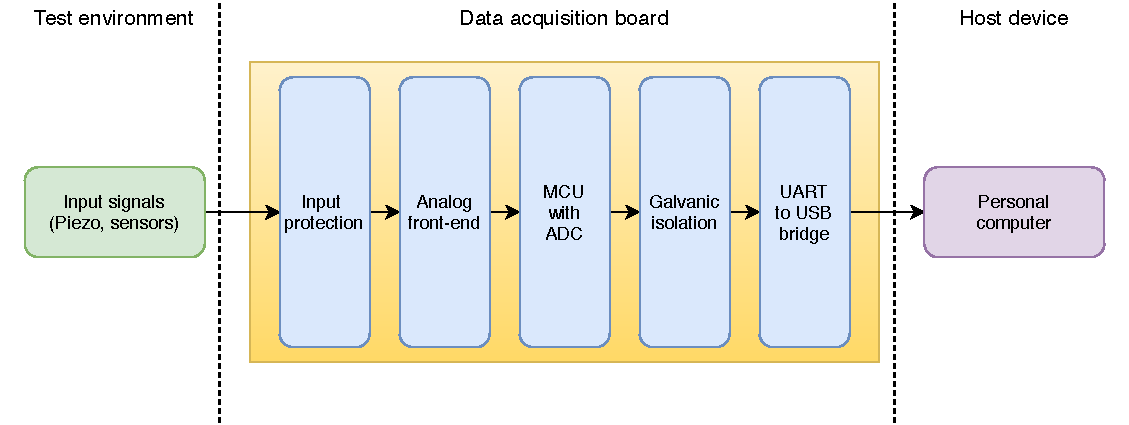
\includegraphics[scale=0.8]{measurement_setup_overview.pdf}
\caption{Measurement setup overview}
\label{fig:meas_overview}
\end{figure}

\subsection{Design requirements}
The first step of the design process is to determine desired input ratings as well as data acquisition capabilities. The piezoelectric device used in this project would be the major signal source during all experiments. Its datasheet \cite{PPA} does not state any fixed maximum ratings. Instead, it provides exemplary results obtained by varying acceleration amplitude, frequency, tip mass and load resistance - see Table \ref{tab:ppapower}.\par

\begin{table}[ht!]
\centering
\begin{tabular}{|c|c|c|c|c|c|c|}
\hline
\multicolumn{1}{|c|}{\textbf{\begin{tabular}[c]{@{}c@{}}Acceler.\\ ampl. $(g)$\end{tabular}}} & \multicolumn{1}{c|}{\textbf{\begin{tabular}[c]{@{}c@{}}Freq.\\ $(Hz)$\end{tabular}}} & \multicolumn{1}{c|}{\textbf{\begin{tabular}[c]{@{}c@{}}Tip mass\\ $(gram)$\end{tabular}}} & \multicolumn{1}{c|}{\textbf{\begin{tabular}[c]{@{}c@{}}RMS\\ power $(mW)$\end{tabular}}} & \multicolumn{1}{c|}{\textbf{\begin{tabular}[c]{@{}c@{}}RMS\\ voltage $(V)$\end{tabular}}} & \multicolumn{1}{c|}{\textbf{\begin{tabular}[c]{@{}c@{}}RMS\\ current $(mA)$\end{tabular}}} & \textbf{\begin{tabular}[c]{@{}c@{}}Load\\ $(k\Omega)$\end{tabular}} \\ \hline
0.25                                                                                                 & 132                                                                                    & 0.0                                                                                     & 0.1                                                                                    & 1.1                                                                                     & 0.1                                                                                      & 17.9                                                                 \\
0.50                                                                                                 & 131                                                                                    & 0.0                                                                                     & 0.2                                                                                    & 1.9                                                                                     & 0.1                                                                                      & 18.3                                                                 \\
1.00                                                                                                 & 131                                                                                    & 0.0                                                                                     & 0.7                                                                                    & 3.4                                                                                     & 0.2                                                                                      & 15.7                                                                 \\
2.00                                                                                                 & 129                                                                                    & 0.0                                                                                     & 2.2                                                                                    & 5.4                                                                                     & 0.4                                                                                      & 13.0                                                                 \\ \hline
0.25                                                                                                 & 60                                                                                     & 1.9                                                                                     & 0.1                                                                                    & 2.9                                                                                     & 0.0                                                                                      & 61.0                                                                 \\
0.50                                                                                                 & 60                                                                                     & 1.8                                                                                     & 0.5                                                                                    & 3.3                                                                                     & 0.2                                                                                      & 20.8                                                                 \\
1.00                                                                                                 & 60                                                                                     & 1.7                                                                                     & 1.8                                                                                    & 7.1                                                                                     & 0.3                                                                                      & 28.6                                                                 \\ \hline
0.25                                                                                                 & 22                                                                                     & 22.8                                                                                    & 1.4                                                                                    & 9.0                                                                                     & 0.1                                                                                      & 60.4                                                                 \\
0.50                                                                                                 & 22                                                                                     & 22.8                                                                                    & 4.4                                                                                    & 17.3                                                                                    & 0.3                                                                                      & 67.6                                                                 \\ \hline

\end{tabular}
\caption{Exemplary piezoelectric harvester response. Data from PPA-1001 datasheet \cite{PPA}}
\label{tab:ppapower}
\end{table}

As mentioned in the previous paragraph, there is no constrained area in terms of vibration frequency and level stated by the manufacturer. Based on the data presented in the Table \ref{tab:ppapower}, the designer is relatively free to determine the operating frequency range as well as input signal range recorded at at the harvester's output. When considering bandwidth and sampling rate, it is important to take into account the Nyquist criterion. It states that the sampling rate has to be twice the highest frequency in the signal \cite{ElEx}. Assuming maximum vibration frequency of 500Hz, more than 1000 samples per second need to be captured.
\par

Of course, this sampling rate only allows to reproduce an incoming signal (sinusoidal wave) as a corrupted triangle, since there is not enough data points to accurately reflect the sine shape. To solve this problem, the sampling rate should be increased by factor of 5 or so, what ultimately yields at least 5000 samples per second (sps). To illustrate the problem, Figure \ref{fig:nyquist} is introduced. It can be easily seen that sampling rate as high as twice the input signal frequency is definitely not enough. Having said that, the minimum expected sampling rate is to be at least 5000 sps.
\par

\begin{figure}[h!]
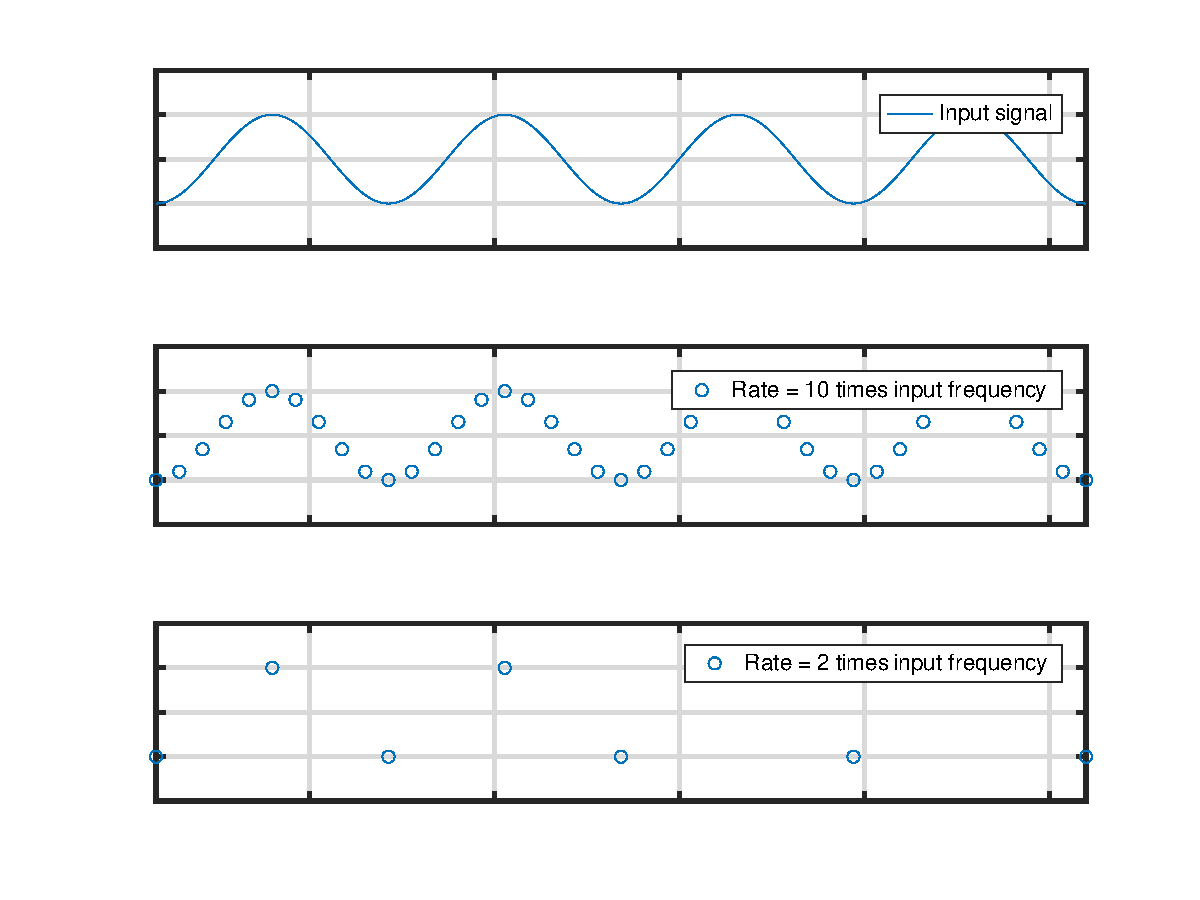
\includegraphics[scale=0.75]{nyquist.pdf}
\caption{Captured waveform versus sampling rate}
\label{fig:nyquist}
\end{figure}

It is likely that the microcontroller used in the data logger would use some kind of a serial communication protocol. Assuming that more than one signal is recorded at the time and the baud rate is fixed at the same level, the maximum input signal frequency would be divided by the number of active channels. For example, for 2 channel measurement, the maximum input signal frequency is 250Hz and so on.
\par

One of the previous paragraphs mentioned the piezoelectric harvester as the main input signal source. Knowing that the device produces a sinusoidal output, the analog front-end has to be able to capture AC signals, preferably of a relatively high amplitude. This requirements force the designer to develop symmetrical power supply for the input section as well as the circuitry allowing to add offset to the signal before it reaches the ADC input. A reason is that the ADC of the microcontroller is likely to accept only unipolar signals within tightly specified range. Remaining channels would be able to interface DC signals only, what makes them suitable for external sensors such as the accelerometer.
\par

When considering the maximum input signal level, one has to note that it should not exceed supply voltage of operational amplifier used in the input section. In case of the designed device, the power supply would be industrial $\pm{15}VDC$, as it helps to maintain compatibility with wide range of available operational amplifiers. Based on the last sentence, the maximum input voltage is specified to $\pm{15}V$ for the AC input and $+{15}V$ for DC inputs. In order to assure proper operating conditions for the analog-front end, an additional input protection is to be provided.
\par
There are two last aspect that need some care. The first one is the resolution of the ADC that would be used to capture the incoming signal. The second one is the input impedance of input channels.
\par
As to the first point, it is useful to have a look at technical details of commonly available oscilloscopes, since they can be treated as a nice reference. Most of them utilize 8 or 10-bit ADCs, mostly because of bandwidth requirements as well as the sampling time. In case of this design, the bandwidth is significantly reduced, what allows to look for a bit more resolution, of course still bearing in mind that all the processes are handled by one modest microcontroller. Putting it all together, an 14-bit ADC is going to be a desired data converter.
\par
The last point relates to the impedance of analog inputs. Piezoelectric harvesters are high output impedance devices \cite{EnHv1}, therefore it is desirable to maintain as high input impedance of the analog front-end as possible, in order not to disturb the incoming signal. There are two potential problems that may occur when designing the input stage. As it can be guessed, the input signal has to be divided before it gets to the analog-to-digital converter. The easiest way to go is to put a voltage divider directly at the output of the harvester. Unfortunately, this circuit would have a significant influence on the impedance seen from piezo generator's output terminals, thus posing a risk of changing its operating conditions. To deal with this problem, the incoming signal is to be buffered before any further processing. This is where low input bias current operational amplifiers would come in handy. The second risk is related to the protection circuitry attached to input terminals. Once the input signal gets to high, it would be clamped in order to protect the data acquisition board. Unhappily, it would also disturb the measured object due to rapid change of the impedance seen at mentioned harvester's output terminals. The only way to deal with this issue is to provide relatively high supply voltage for buffering amplifiers and adjust the load as to meet the input voltage requirements.
\par

As a summary of design considerations included in this subsection, Table \ref{tab:requirements} has been created.
\begin{table}[ht!]
\begin{tabular}{|l|c|}
\hline
\textbf{Requirement}              & \textbf{Value} \\ \hline
Max. input signal frequency (Sine) & 500Hz          \\ \hline
Min. sampling rate                 & 5000sps        \\ \hline
Min. ADC resolution                & 14-bit         \\ \hline
Max. input voltage range (p-p)     & 15V            \\ \hline
Input impeadnce                    & TBD            \\ \hline
\end{tabular}
\caption{Summary of requirements for the data acquisition board}
\label{tab:requirements}
\end{table}
\par

\subsection{Accelerometer board}
As it has been previously mentioned, is is necessary to constantly monitor vibration level during all the experiments. These measurements will be a reference for the results obtained using the piezoelectric harvester, as they easily allow to correlate generated power and current vibration level.
\par

The piezoelectric beam used throughout the research is mounted in a 3D-printed holder provided by the device manufacturer. Apart from a proper fit, it allows to attach some external electronics by means using nice mounting holes. It is worth to take advantage of this feature, therefore designed electronics would be compatible with the handler.
\par

\subsubsection{Most important parameters of the accelerometer}
As to the electrical and electromechanical properties of the accelerometer, there are a few aspects that should be highlighted. The first one is the measurement range. By checking the maximum acceleration of the beam, it is possible to estimate required range for the sought integrated circuit. Next, the frequency response and output signal type need to be determined. Frequency response describes the measurement resolution that could be understand as the smallest detectable acceleration \cite{accel_params}. By mentioning the type of the output signal, it was intended to distinguish between analog and digital output types. It is planned to synchronize the accelerometer output with the piezoelectric cantilever response, so the analog output is more suitable and easier to use.
\par
Harvester's datasheet \cite{PPA} does not mention the exact upper limit of allowed vibration level. According to the Table \ref{tab:ppapower}, the maximum acceleration amplitude mentioned by the manufacturer is 2g. Without any additional information, it is reasonable to treat this value as the upper acceleration limit. The same applies to the frequency response, which is also not described precisely. Again, Table \ref{tab:ppapower} states the maximum operation frequency at the level of 132Hz. In this case, the minimum acceptable bandwidth of the accelerometer would be roughly 200Hz. As it was mentioned in the previous paragraph, it is intended to use the analog output accelerometer. A summary of the above-mentioned choices is presented in the Table \ref{tab:accel_requirements}.

\begin{table}[ht!]
\begin{tabular}{|l|c|}
\hline
\textbf{Requirement}            & \textbf{Value} \\ \hline
Max. acceleration value  		& 2g         \\ \hline
Max. operating frequency        & 300Hz        \\ \hline
Output type             		& Analog         \\ \hline
\end{tabular}
\caption{Summary of requirements for the accelerometer}
\label{tab:accel_requirements}
\end{table}
\par

\subsubsection{Selection of the integrated circuit}
After a thorough market research, a proper device has been found - see Table \ref{tab:adxl_params}. Apart from parameters listed in the table, the selected accelerometer has the following features: small SMD package, 3.3V supply operation, low power consumption and tunable bandwidth filters for every axis. Moreover, it exhibits non-linearity at a level of 0.3$\%$ \cite{ADXL}.

\begin{table}[ht!]
\begin{tabular}{|l|c|}
\hline
\textbf{Parameter}		& \textbf{Value} 	\\ \hline
Model  					& ADXL335         	\\ \hline
Manufacturer        	& Analog devices	\\ \hline
Output type           	& Analog  			\\ \hline
Max. acceleration value &  $\pm{3}g$		\\ \hline
Bandwidth 				&  up to 1600Hz		\\ \hline
\end{tabular}
\caption{Parameters of the selected parameter - taken from the datasheet \cite{ADXL}}
\label{tab:adxl_params}
\end{table}

\begin{figure}[ht!]
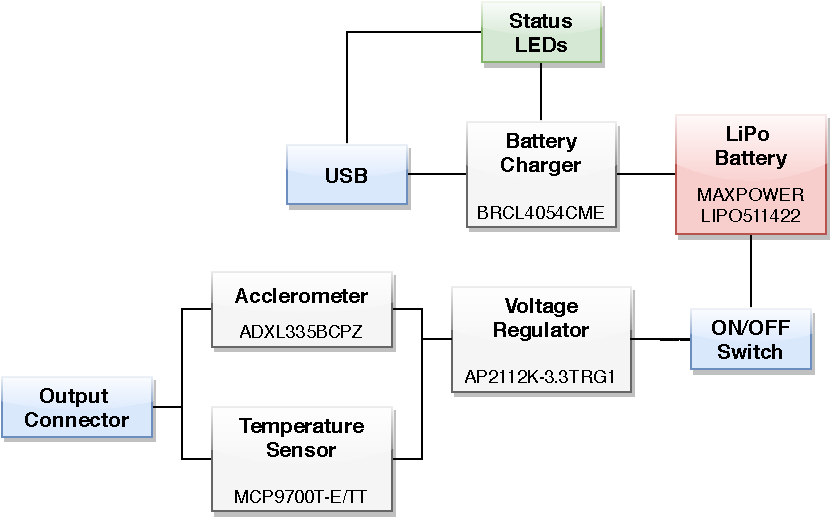
\includegraphics[scale=1]{accel.pdf}
\caption{Accelerometer board diagram}
\label{fig:accel_diagram}
\end{figure}

\begin{figure}[ht!]
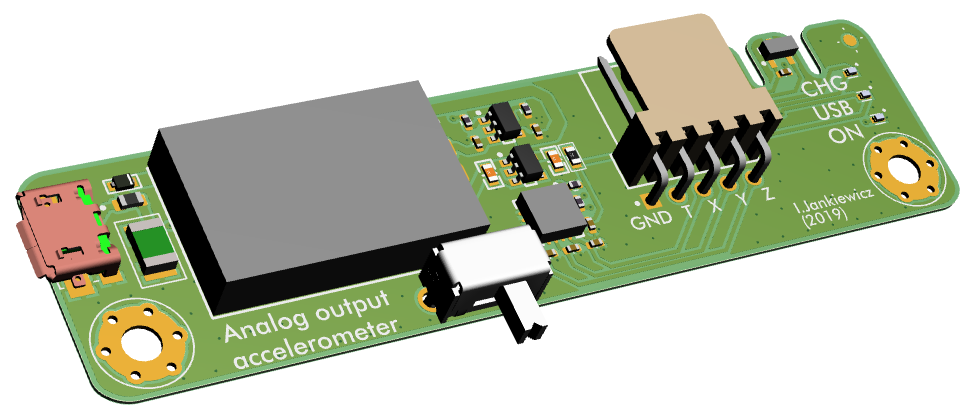
\includegraphics[scale=0.6]{accelerometer1.png}
\caption{Accelerometer board top side view}
\label{fig:accel1}
\end{figure}

\begin{figure}[ht!]
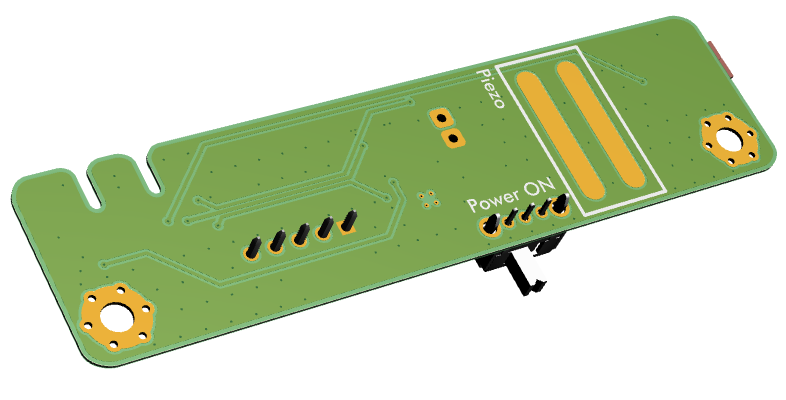
\includegraphics[scale=0.7]{accelerometer2.png}
\caption{Accelerometer board bottom side view}
\label{fig:accel2}
\end{figure}
\par 

\newpage

\bibliography{bibliography} 
\bibliographystyle{ieeetr}

\end{document}
